\documentclass[a4paper,10pt]{report}
\usepackage[utf8x]{inputenc}
\usepackage{amsmath}
\usepackage{amssymb}
\usepackage{amsfonts}
\usepackage{mathrsfs}
% \usepackage{natbib}
 \usepackage{graphicx} % figuras
% \usepackage[export]{adjustbox} % loads also graphicx
% \usepackage{float}
% \usepackage[font=footnotesize]{caption}
\usepackage{wrapfig}
% Title Page
\title{}
\author{}


\begin{document}

On the interval (0,1) we consider a steady-state convection-diffusion-reaction equation, with homogeneous Neumann boundary conditions:

\begin{align}\label{eq:1}
 -D\frac{d^2u}{dx^2}+\lambda u= f(x), \\
 -D\frac{du}{dx}(0)=0, \qquad -D\frac{du}{dx}(1)=0.
\end{align}
\begin{enumerate}
 \item{Assignment 1} Derive the $weak$ formulation. \\
 For this, we multiply Equation \eqref{eq:1} by the basis functions $\phi$ and integrate over the domain.\\
 \begin{equation}\label{eq:2}
 \int_{0}^{1} -D\phi\frac{d^2u}{dx^2}+\lambda \phi u dx= \int_{0}^{1}\phi f(x)dx 
\end{equation}
  \begin{align*}
 =\int_{0}^{1} -D\left[\frac{du}{dx}\left(\phi\frac{du}{dx}\right)-\frac{d\phi}{dx}\frac{du}{dx}+\lambda \phi u \right]dx=\\
 \int_{0}^{1} -D\mathbf{n}\cdot \phi\frac{du}{dx} ds+\int_{0}^{1}D\left[\frac{d\phi}{dx}\frac{du}{dx}+\lambda \phi u \right]dx
\end{align*}
But using Equation \eqref{eq:1} (bc) the first term above is zero, then we have:
 \begin{equation}\label{eq:3}
\int_{0}^{1}\left[D\frac{d\phi}{dx}\frac{du}{dx}+\lambda \phi u \right]dx= \int_{0}^{1}\phi f(x)dx
\end{equation}
\item{Assignment 2} Write the Galerkin formulation of the weak form as derived
in the previous assignment for a general number of elements given by n (hence
$x_n = 1$). Give the Galerkin equations, that is, the linear system in terms of
\begin{equation}\label{eq:4}
S\bar{u} = \bar{f},
 \end{equation}
all expressed in the basis-functions, $f(x)$, $\lambda$ and $D$.\\
For the Galerkin formulation we approximate ${u}$ with the basis functions $\phi_j$ as:
$$u(x)\sim \sum_{j=1}^na_j\phi_j(x).$$
Approximating $u$ and substituting $\phi=\phi_i$ in Equation \eqref{eq:3} we have:
 \begin{equation}\label{eq:5}
\sum_{j=1}^na_j\int_{0}^{1}\left[D\frac{d\phi_i}{dx}\frac{d\phi_j}{dx}+\lambda \phi_i \phi_j \right]dx= \int_{0}^{1}\phi_i f(x)dx
\end{equation}
Then 
\begin{align*}
S_{ij}^{e_k}&=a_j\int_{e_k}\left[D\frac{d\phi_i}{dx}\frac{d\phi_j}{dx}+\lambda \phi_i \phi_j \right]dx, \qquad &S_{ij}=\sum_{k=1}^{nel}S_{ij},\\
f_i^{e_k}&=\int_{e_k}\phi_i f(x)dx, \qquad &f_i=\sum_{k=1}^{nel}f_i^{e_k}.
\end{align*}
\item{Assignment 3} Write a matlab routine, called GenerateMesh.m that gener-
ates an equidistant distribution of meshpoints over the interval [0, 1], where
$x_1 = 0$ and $x_n = 1$ and $h =\frac{1}{n−1}$. You may use x = linspace(0,1,n).

\begin{table}[!h]\centering

\begin{tabular}{ |l| } 
\hline
\textbf{Algorithm 1}\\
\hline
\hspace{0.5cm}function [x]=GenerateMesh(n)\\
\hspace{1cm}x = linspace(0,1,n);\\
\hspace{0.5cm}end\\
\hline
\end{tabular}
\end{table}

\item{Assignment 4} Write a routine, called GenerateTopology.m, that generates
a two dimensional array, called elmat, which contains the indices of the ver-
tices of each element, that is
\begin{align*}
&elmat(i, 1) = i. \qquad for i ∈ {1, . . . , n − 1}.\\
&elmat(i, 2) = i + 1
\end{align*}
Next we compute the element matrix $S_{elem}$. In this case, the matrix is the
same for each element, that is, if we consider element $e_i$.

\begin{table}[!h]
\centering
\begin{tabular}{ |l| } 
\hline
\textbf{Algorithm 1}\\
\hline
\hspace{0.5cm}function [elmat] = GenerateTopology(n)\\
\hspace{0.5cm}for i = 1 : n-1;\\
\hspace{1cm}elmat(i, 1) = i;\\
\hspace{1cm}elmat(i, 2) = i + 1;\\
\hspace{0.5cm}end\\
\hspace{0.5cm}end\\
\hline
\end{tabular}
\end{table}


\item{Assignment 5} Compute the element matrix, $S_{elem}$ over a generic line element $e_k$.\\
For each element we have the following marix:

\begin{equation*}
 S^{e_k}=
\begin{bmatrix}
    \int_{e_k}D\phi'_{k-1}\phi'_{k-1}+\lambda \phi_{k-1} \phi_{k-1} dx & \int_{e_k}D\phi'_{k-1}\phi'_k+\lambda \phi_{k-1} \phi_k dx \\
    &\\
\int_{e_k}D\phi'_k\phi'_{k-1}+\lambda \phi_k \phi_{k-1} dx& \int_{e_k}D\phi'_k\phi'_k+\lambda \phi_k \phi_k dx
\end{bmatrix}
\end{equation*}
According to Holland and Bell's Theorem, we have:
\begin{align*}
     &\int_{e_k}\phi_{k-1} \phi_{k-1} dx =\frac{||x_k-x_{k-1}||}{3}\\
      &\int_{e_k}\phi_{k} \phi_{k-1} dx =\frac{||x_k-x_{k-1}||}{6} \\
      &\int_{e_k}\phi'_{k-1}\phi'_{k-1} dx=\frac{1}{||x_k-x_{k-1}||}\\
   &\int_{e_k}\phi'_{k-1}\phi'_{k} dx=-\frac{1}{||x_k-x_{k-1}||}
\end{align*}
Then we have 
\begin{equation*}
 S^{e_k}=
\begin{bmatrix}
  D\frac{1}{||x_k-x_{k-1}||}+\lambda \frac{||x_k-x_{k-1}||}{3} &   -D\frac{1}{||x_k-x_{k-1}||}+\lambda \frac{||x_k-x_{k-1}||}{6} \\
    &\\
-  D\frac{1}{||x_k-x_{k-1}||}+\lambda \frac{||x_k-x_{k-1}||}{6}&   D\frac{1}{||x_k-x_{k-1}||}+\lambda \frac{||x_{k}-x_{k-1}||}{3}
\end{bmatrix}
\end{equation*}
But $||x_k-x_{k-1}|| = h=\frac{1}{n-1}$ then 
\begin{equation*}
 S^{e_k}=
\begin{bmatrix}
  D\frac{1}{h}+\lambda \frac{h}{3} &   -D\frac{1}{h}+\lambda \frac{h}{6} \\
    &\\
-  D\frac{1}{h}+\lambda \frac{h}{6}&   D\frac{1}{h}+\lambda \frac{h}{3}
\end{bmatrix}
\end{equation*}

\item{Assignment 6} Write a matlab routine, called GenerateElementMatrix.m,
in which $S_{elem}$ (2 x 2-matrix) is generated. 
Subsequently, we are going to sum the connections of the vertices in each
element matrix, over all the elements. The result is an n-by-n matrix, called
S.

\begin{table}
\begin{tabular}{ |l| } 
\hline
\textbf{Algorithm 3}\\
\hline
\hspace{0.5cm}function [Selem]=GenerateElementMatrix(D,l,n)\\
\hspace{1cm}h = 1/(n-1);\\
\hspace{1cm}Selem(1,1) = D/h + l*h/3;\\
\hspace{1cm}Selem(1,2) = -D/h + l*h/6;\\
\hspace{1cm}Selem(2,1) = -D/h + l*h/6;\\
\hspace{1cm}Selem(2,2) = D/h + l*h/3;\\
\hspace{0.5cm}end\\
\hline
\end{tabular}
\end{table}

\item{Assignment 7} Write a matlab routine, called AssembleMatrix.m, that performs
this summation, such that S is first initialized as a zero n-by-n matrix
and subsequently:\\
\begin{equation} \label{eq:6}
 S(elmat(i, j), elmat(i, k)) = S(elmat(i, j), elmat(i, k)) + Selem(j, k),
\end{equation}
for $ j, k \in \{1, 2\}$ over all elements $i \in \{1, . . . , n − 1\}$. Note that GenerateElementMatrix.m
needs to be called for each element.
Now, you developed a routine for the assembly of the large matrix S from
the element matrices Selem for each element. This procedure is common
for the construction of the large discretization matrices needed in Finite
Element methods. The procedure, using the array elmat looks a bit overdone
and complicated. However, this approach facilitates the application to multi
dimensional problems. The next step is to generate a large right-hand side
vector using the same procedure. First, we need the element vector.

\begin{table}
\begin{tabular}{ |l| } 
\hline
\textbf{Algorithm 4}\\
\hline
\hspace{0.5cm}function [S]=AssembleMatrix(elmat,Selem,n)\\
\hspace{0.5cm}S = zeros(n,n);\\
\hspace{0.5cm}for i = 1 : n-1\\
\hspace{1cm}    for j = 1 : 2\\
\hspace{1.5cm}    for k = 1 : 2\\
 \hspace{2cm}           S(elmat(i, j), elmat(i, k)) = S(elmat(i, j), elmat(i, k))+Selem(j, k);\\
 \hspace{1.5cm}       end\\
\hspace{1cm}end\\
\hspace{0.5cm}end\\
\hspace{0.5cm}end\\
\hline
\end{tabular}
\end{table}

\item{Assignment 8} Compute the element vector over a generic line-element.\\
For this purpose, we proceed as follows

\item{Assignment 9} Implementation of the right-hand vector:\\
\begin{itemize}
 \item[a] Write a matlab routine, called GenerateElementVector.m, that gives
the vector felem (column vector of length 2). in which felem (1) and
felem (2) respectively provide information about node i and node i + 1,
which are the vertices of element $e_i$ . This is needed for all elements.
Use $f (x) = 1$ here.\\
According to Newton-Cotes' Theorem, we have:
\begin{align*}
     &\int_{e_k}\phi_{k-1} f(x)dx =\frac{x_k-x_{k-1}}{2}f(x_k)
\end{align*}

\begin{equation*}
 f_{e_k}=
\begin{bmatrix}
    \int_{e_k}\phi_{k-1} f(x)dx \\\\
\int_{e_k}\phi_k f(x)dx
\end{bmatrix}
\end{equation*}
Then, for each element we have
\begin{equation*}
 f_{e_k}=\frac{h}{2}
\begin{bmatrix}
    f(x_{k-1})\\\\
 f(x_{k})
\end{bmatrix}=\frac{h}{2}
\begin{bmatrix}
    1\\\\
 1
\end{bmatrix}
\end{equation*}

\begin{table}
\begin{tabular}{ |l| } 
\hline
\textbf{Algorithm 5}\\
\hline
\hspace{0.5cm}function [felem]=GenerateElementVector(n)\\
\hspace{0.5cm}h = 1 / (n-1);\\
\hspace{0.5cm}for i=1:n-1\\
\hspace{0.5cm}felem(1,i) = (h/2)*fn(x(i));\\
\hspace{0.5cm}felem(2,i) = (h/2)*fn(x(i+1));\\
\hspace{0.5cm}end\\
\hspace{0.5cm}end\\
\hline
\end{tabular}
\end{table}

\item[b] Write a matlab routine, called AssembleVector.m, that performs the
following summation after setting $f = zeros(n, 1)$:
\begin{equation}\label{eq:6}
 f (elmat(i, j)) = f (elmat(i, j)) + felem (j),
\end{equation}
for $j \in \{1, 2\}$ over all elements $i \in \{1, . . . , n − 1\}$.

\begin{table}
\begin{tabular}{ |l| } 
\hline
\textbf{Algorithm 6}\\
\hline
\hspace{0.5cm}[f]=AssembleVector(felem,elmat,n)\\
\hspace{0.5cm}f=zeros(n,1);\\
\hspace{0.5cm}for i=1:n-1\\
\hspace{1cm}for j=1:2\\
\hspace{1.5cm}f(elmat(i,j)) = f(elmat(i,j)) + felem(j,i);\\
\hspace{1cm}end\\
\hspace{0.5cm}end\\
\hspace{0.5cm}end\\
\hline
\end{tabular}
\end{table}

\end{itemize}

\item{Assignment 10} Run the assembly routines to get the matrix $S$ and vector
$f$ for $n = 100$.

\item{Assignment 11} Write the main program that gives the finite-element solution. Call the main program femsolve1d.m. 

\begin{table}
\begin{tabular}{ |l| } 
\hline
\textbf{Algorithm 7}\\
\hline
\hspace{0.5cm}clear all\\
\hspace{0.5cm}[x] = GenerateMesh(n);\\
\hspace{0.5cm}[elmat] = GenerateTopology(n);\\
\hspace{0.5cm}[Selem] = GenerateElementMatrix(D,lambda,n);\\
\hspace{0.5cm}[S] = AssembleMatrix(elmat,Selem,n);\\
\hspace{0.5cm}[felem] = GenerateElementVector(n,fn,x(1:2));\\
\hspace{0.5cm}[f] = AssembleVector(felem,elmat,n);\\
\hspace{0.5cm} $u = S\backslash f$;\\
\hspace{0.5cm}plot(x,u)\\
\hline
\end{tabular}
\end{table}


\item{Assignment 12} Compute the Finite Element solution u for $f (x) = 1$, $D =
1$, $\lambda = 1$ and $n = 100$ by using $u = S\backslash f$ in matlab. Plot the solution. Is this
what you would expect?


\begin{table}
\begin{tabular}{ |l| } 
\hline
\textbf{Algorithm 7b}\\
\hline
\hspace{0.5cm}clear all\\
\hspace{0.5cm}n = 100;\\
\hspace{0.5cm}D = 1;\\
\hspace{0.5cm}lambda = 1;\\
\hspace{0.5cm}fn = @(x) 1;\\
\hspace{0.5cm}[x] = GenerateMesh(n);\\
\hspace{0.5cm}[elmat] = GenerateTopology(n);\\
\hspace{0.5cm}[Selem] = GenerateElementMatrix(D,lambda,n);\\
\hspace{0.5cm}[S] = AssembleMatrix(elmat,Selem,n);\\
\hspace{0.5cm}[felem] = GenerateElementVector(n,fn,x);\\
\hspace{0.5cm}[f] = AssembleVector(felem,elmat,n);\\
\hspace{0.5cm} $u = S\backslash f$;\\
\hspace{0.5cm}plot(x,u)\\
\hline
\end{tabular}
\end{table}
\begin{figure}
\centering 
\vspace{-10pt}
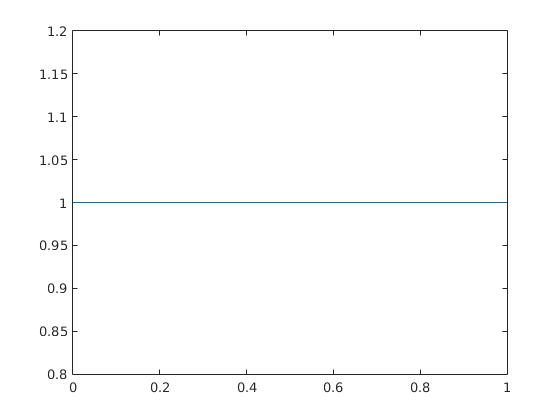
\includegraphics[width=8cm,height=8cm,keepaspectratio]{result1.jpg}
 %\vspace{-25pt}
\caption{ Result $f (x) = 1$.}\label{fig:hep_2}
\vspace{-10pt}
\end{figure} 



\item{Assignment 13} Choose $f (x) = sin(20x)$, do some experiments with several
values of n (n = 10, 20, 40, 80 160). Plot the solutions for the various
numbers of gridnodes in one plot. Explain what you see.
\begin{table}
\begin{tabular}{ |l| } 
\hline
\textbf{Algorithm 7c}\\
\hline
\hspace{0.5cm}clear all\\
\hspace{0.5cm}close all\\
\hspace{0.5cm}t = 0;\\
\hspace{0.5cm}for n = [10 20 40 80 160]\\
\hspace{1cm}n = 100;\\
\hspace{1cm}D = 1;\\
\hspace{1cm}lambda = 1;\\
\hspace{1cm}fn = @(x) sin(20*x);\\
\hspace{1cm}[x] = GenerateMesh(n);\\
\hspace{01cm}[elmat] = GenerateTopology(n);\\
\hspace{1cm}[Selem] = GenerateElementMatrix(D,lambda,n);\\
\hspace{1cm}[S] = AssembleMatrix(elmat,Selem,n);\\
\hspace{1cm}[felem] = GenerateElementVector(n,fn,x);\\
\hspace{1cm}[f] = AssembleVector(felem,elmat,n);\\
\hspace{1cm} $u = S\backslash f$;\\
\hspace{1cm}plot(x,u)\\
\hspace{1cm}hold on\\
\hspace{1cm}t = t + 1;\\
\hspace{1cm}name\{t\}=num2str(n);\\
\hspace{0.5cm}end\\
\hspace{0.5cm}legend(['n=' name\{1\}],['n=' name\{2\}],['n=' name\{3\}],['n=' name\{4\}],['n=' name\{5\}])\\
\hline
\end{tabular}
\end{table}
\begin{figure}
\centering 
\vspace{-10pt}
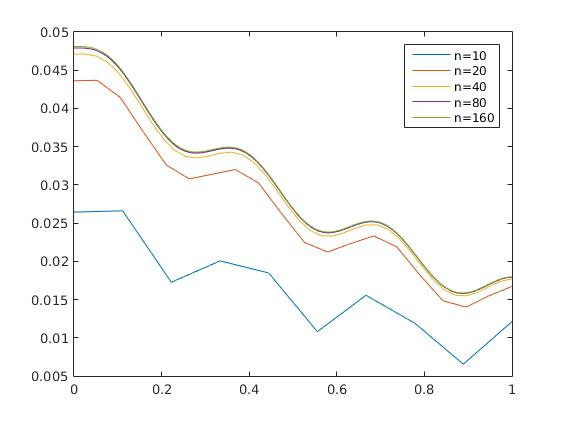
\includegraphics[width=8cm,height=8cm,keepaspectratio]{result.jpg}
 %\vspace{-25pt}
\caption{ Results $f (x) = sin(20x)$.}\label{fig:hep_2}
\vspace{-10pt}
\end{figure} 
\end{enumerate}



\end{document}          
